% Fantastic Personas and Where to Find Them — Research Poster v2
% 24x36 inch portrait, beamerposter
\documentclass[final,t]{beamer}
\usepackage[size=custom,width=60.96,height=91.44,scale=1.0,orientation=portrait]{beamerposter}

\setbeamertemplate{navigation symbols}{}
\setbeamertemplate{headline}{}
\setbeamertemplate{footline}{}

\usepackage{graphicx}
\usepackage{booktabs}
\usepackage{enumitem}
\usepackage{amsmath}
\usepackage{fontspec}
\usepackage{tcolorbox}
\usepackage{ragged2e}

\setbeamersize{text margin left=22mm, text margin right=22mm}

\setsansfont{Helvetica Neue}[
  BoldFont={Helvetica Neue Bold},
  ItalicFont={Helvetica Neue Italic},
]
\renewcommand{\familydefault}{\sfdefault}

\definecolor{posterindigo}{HTML}{2C3E6B}
\definecolor{postergold}{HTML}{E8A838}
\definecolor{posterslate}{HTML}{4A6FA5}
\definecolor{posterbg}{HTML}{FAFAFA}
\definecolor{postergreen}{HTML}{2EAA6F}
\definecolor{posterred}{HTML}{E85D5D}
\definecolor{posterlight}{HTML}{E8EDF5}
\definecolor{posterdark}{HTML}{1A2744}

\setbeamercolor{background canvas}{bg=posterbg}
\setbeamercolor{block title}{fg=white,bg=posterslate}
\setbeamercolor{block body}{fg=posterdark,bg=white}
\setbeamercolor{block alerted title}{fg=white,bg=posterindigo}
\setbeamercolor{block alerted body}{fg=posterdark,bg=white}

\setbeamertemplate{block begin}{
  \vskip 3pt
  \begin{beamercolorbox}[rounded=true,shadow=false,
    leftskip=5mm,colsep*=.5ex,sep=3mm]{block title}
    \usebeamerfont{block title}\insertblocktitle
  \end{beamercolorbox}
  \vskip-2pt
  \begin{beamercolorbox}[rounded=true,shadow=false,
    colsep*=.5ex,sep=3.5mm,vmode]{block body}
    \usebeamerfont{block body}\justifying\setlength{\parskip}{2pt}
}
\setbeamertemplate{block end}{
  \end{beamercolorbox}
  \vskip 3pt
}

\setbeamerfont{block title}{size=\large,series=\bfseries}
\setbeamerfont{block body}{size=\small}

\setbeamertemplate{itemize items}[circle]
\setbeamercolor{item}{fg=posterslate}

\newtcolorbox{hlbox}{
  colback=posterlight, colframe=posterslate!40,
  boxrule=0.4pt, arc=3pt, left=4pt, right=4pt, top=2pt, bottom=2pt,
  fontupper=\color{posterdark}\small
}

\graphicspath{{figures/}{../figures/role-figures/}{../figures/christina-figures/}}

\begin{document}
\begin{frame}[t]

% ── TITLE ───────────────────────────────────────────────────
\vspace{-7mm}
\begin{beamercolorbox}[wd=\textwidth,rounded=true,shadow=false,
  sep=5mm]{block alerted title}
  \begin{minipage}[c]{0.15\textwidth}
    \centering
    
\includegraphics[width=\linewidth]{mats_white.png}\\[5pt]
    
\includegraphics[width=0.8\linewidth]{gt_computing_white.pdf}\\[5pt]
    \begin{minipage}[t]{0.3\linewidth}\centering
      
\includegraphics[width=\linewidth]{openai_white.pdf}
    \end{minipage}\hfill
    \begin{minipage}[t]{0.3\linewidth}\centering
      
\includegraphics[width=\linewidth]{uiuc_logo.png}
    \end{minipage}\hfill
    \begin{minipage}[t]{0.3\linewidth}\centering
      
\includegraphics[width=\linewidth]{deepmind_white.pdf}
    \end{minipage}
  \end{minipage}%
  \hfill
  \begin{minipage}[c]{0.68\textwidth}
    \centering
    {\fontsize{38}{46}\selectfont\bfseries\color{white}%
      Fantastic Personas and Where to Find Them}\\[4pt]
    {\Large\color{white}%
      Mapping the Geometry of Role Vectors in Activation Space}\\[6pt]
    {\normalsize\color{white}%
      Glenn Matlin$^{1,2}$,\;
      Isaac Song$^{2}$,\;
      M.~R.~Parwani$^{2}$,\;
      E.~T.~Anand$^{3}$,\;
      A.~Theerthala$^{2}$,\;
      A.~Chatterjee$^{4}$,\\[1pt]
      M.~Kostylew$^{1}$,\;
      Y.~G~Shavit$^{1,5}$,\;
      S.~Krier$^{1,6}$,\;
      M.~Riedl$^{2}$}\\[3pt]
    {\small\color{white}%
      $^1$MATS\quad
      $^2$Human-Centered AI Lab, Georgia Tech\quad
      $^3$School of CS, Georgia Tech\quad
      $^4$UIUC\quad
      $^5$OpenAI\quad
      $^6$Google DeepMind}
  \end{minipage}%
  \hfill
  \begin{minipage}[c]{0.15\textwidth}
    \hfill
  \end{minipage}
\end{beamercolorbox}

\vspace{1mm}

% ── COLUMNS (0.28 / 0.36 / 0.28) ───────────────────────────
\begin{columns}[T]

% ══════════════════════════════════════════════════════════
% COLUMN 1
% ══════════════════════════════════════════════════════════
\begin{column}{0.28\textwidth}

\begin{block}{Motivation}
LLMs adopt personas when prompted, and these behavioral shifts
correspond to recoverable directions in activation space [1, 2].
Contrastive steering can manipulate outputs along these
directions [3, 4, 7], though instruction-level persona control
remains unstable across dialog turns [8]. Persona features have
been linked to emergent misalignment [5].

The Persona Selection Model [9] proposes that LLMs learn a
structured persona space during pre-training. \textbf{Can
contrastive extraction recover this structure?}

We extract role vectors for \textbf{275 roles} from
OLMo3-7B-Instruct and analyze the geometry of the resulting
persona space, finding interpretable structure beyond the
previously documented assistant axis [1].
\end{block}

\begin{block}{Method}
For each role, we generate paired responses: one with a
role-specific system prompt and one with no system prompt.
An LLM judge scores both for role alignment (0--100); only
pairs passing a quality threshold are retained.

We compute contrastive activation vectors at layer 16:
\[\vec{v}_{\text{role}} = \vec{a}_{\text{prompted}} - \vec{a}_{\text{baseline}}\]
These 4,096-dim vectors encode the persona direction in
activation space.

\vspace{2pt}
\begin{hlbox}
\renewcommand{\arraystretch}{1.1}
\begin{tabular}{@{}lll@{}}
\toprule
& \textbf{Lu et al.} & \textbf{Ours} \\
\midrule
Extraction & Mean act. & Contrastive diff \\
Filter & None & LLM judge \\
Questions & 230+ & 20--50 \\
Behavior & Assistant-like & 1st-person role \\
Eval & Not done & 5-axis judge \\
Mean sub. & Yes & No \\
\bottomrule
\end{tabular}
\end{hlbox}

\vspace{1pt}
{\scriptsize\textbf{Model:} OLMo3-7B-Instruct\enspace|\enspace
\textbf{Layer:} 16\enspace|\enspace
\textbf{Judge:} GPT-4.1\\
\textbf{Roles:} 275 extracted, 97 evaluated\enspace|\enspace
\textbf{Scale:} 500k+ Q/A pairs}
\end{block}

\begin{block}{Empirical Results}
Steered outputs and the Assistant Axis baseline [1] are each
compared against a prompt-engineered gold persona response
using a 5-axis GPT-4.1 judge: \textit{emotional register,
vocabulary, social dynamic, motivation, worldview}.
A/B ordering randomized; results debiased.

\vspace{2pt}
\begin{minipage}[t]{0.48\linewidth}
  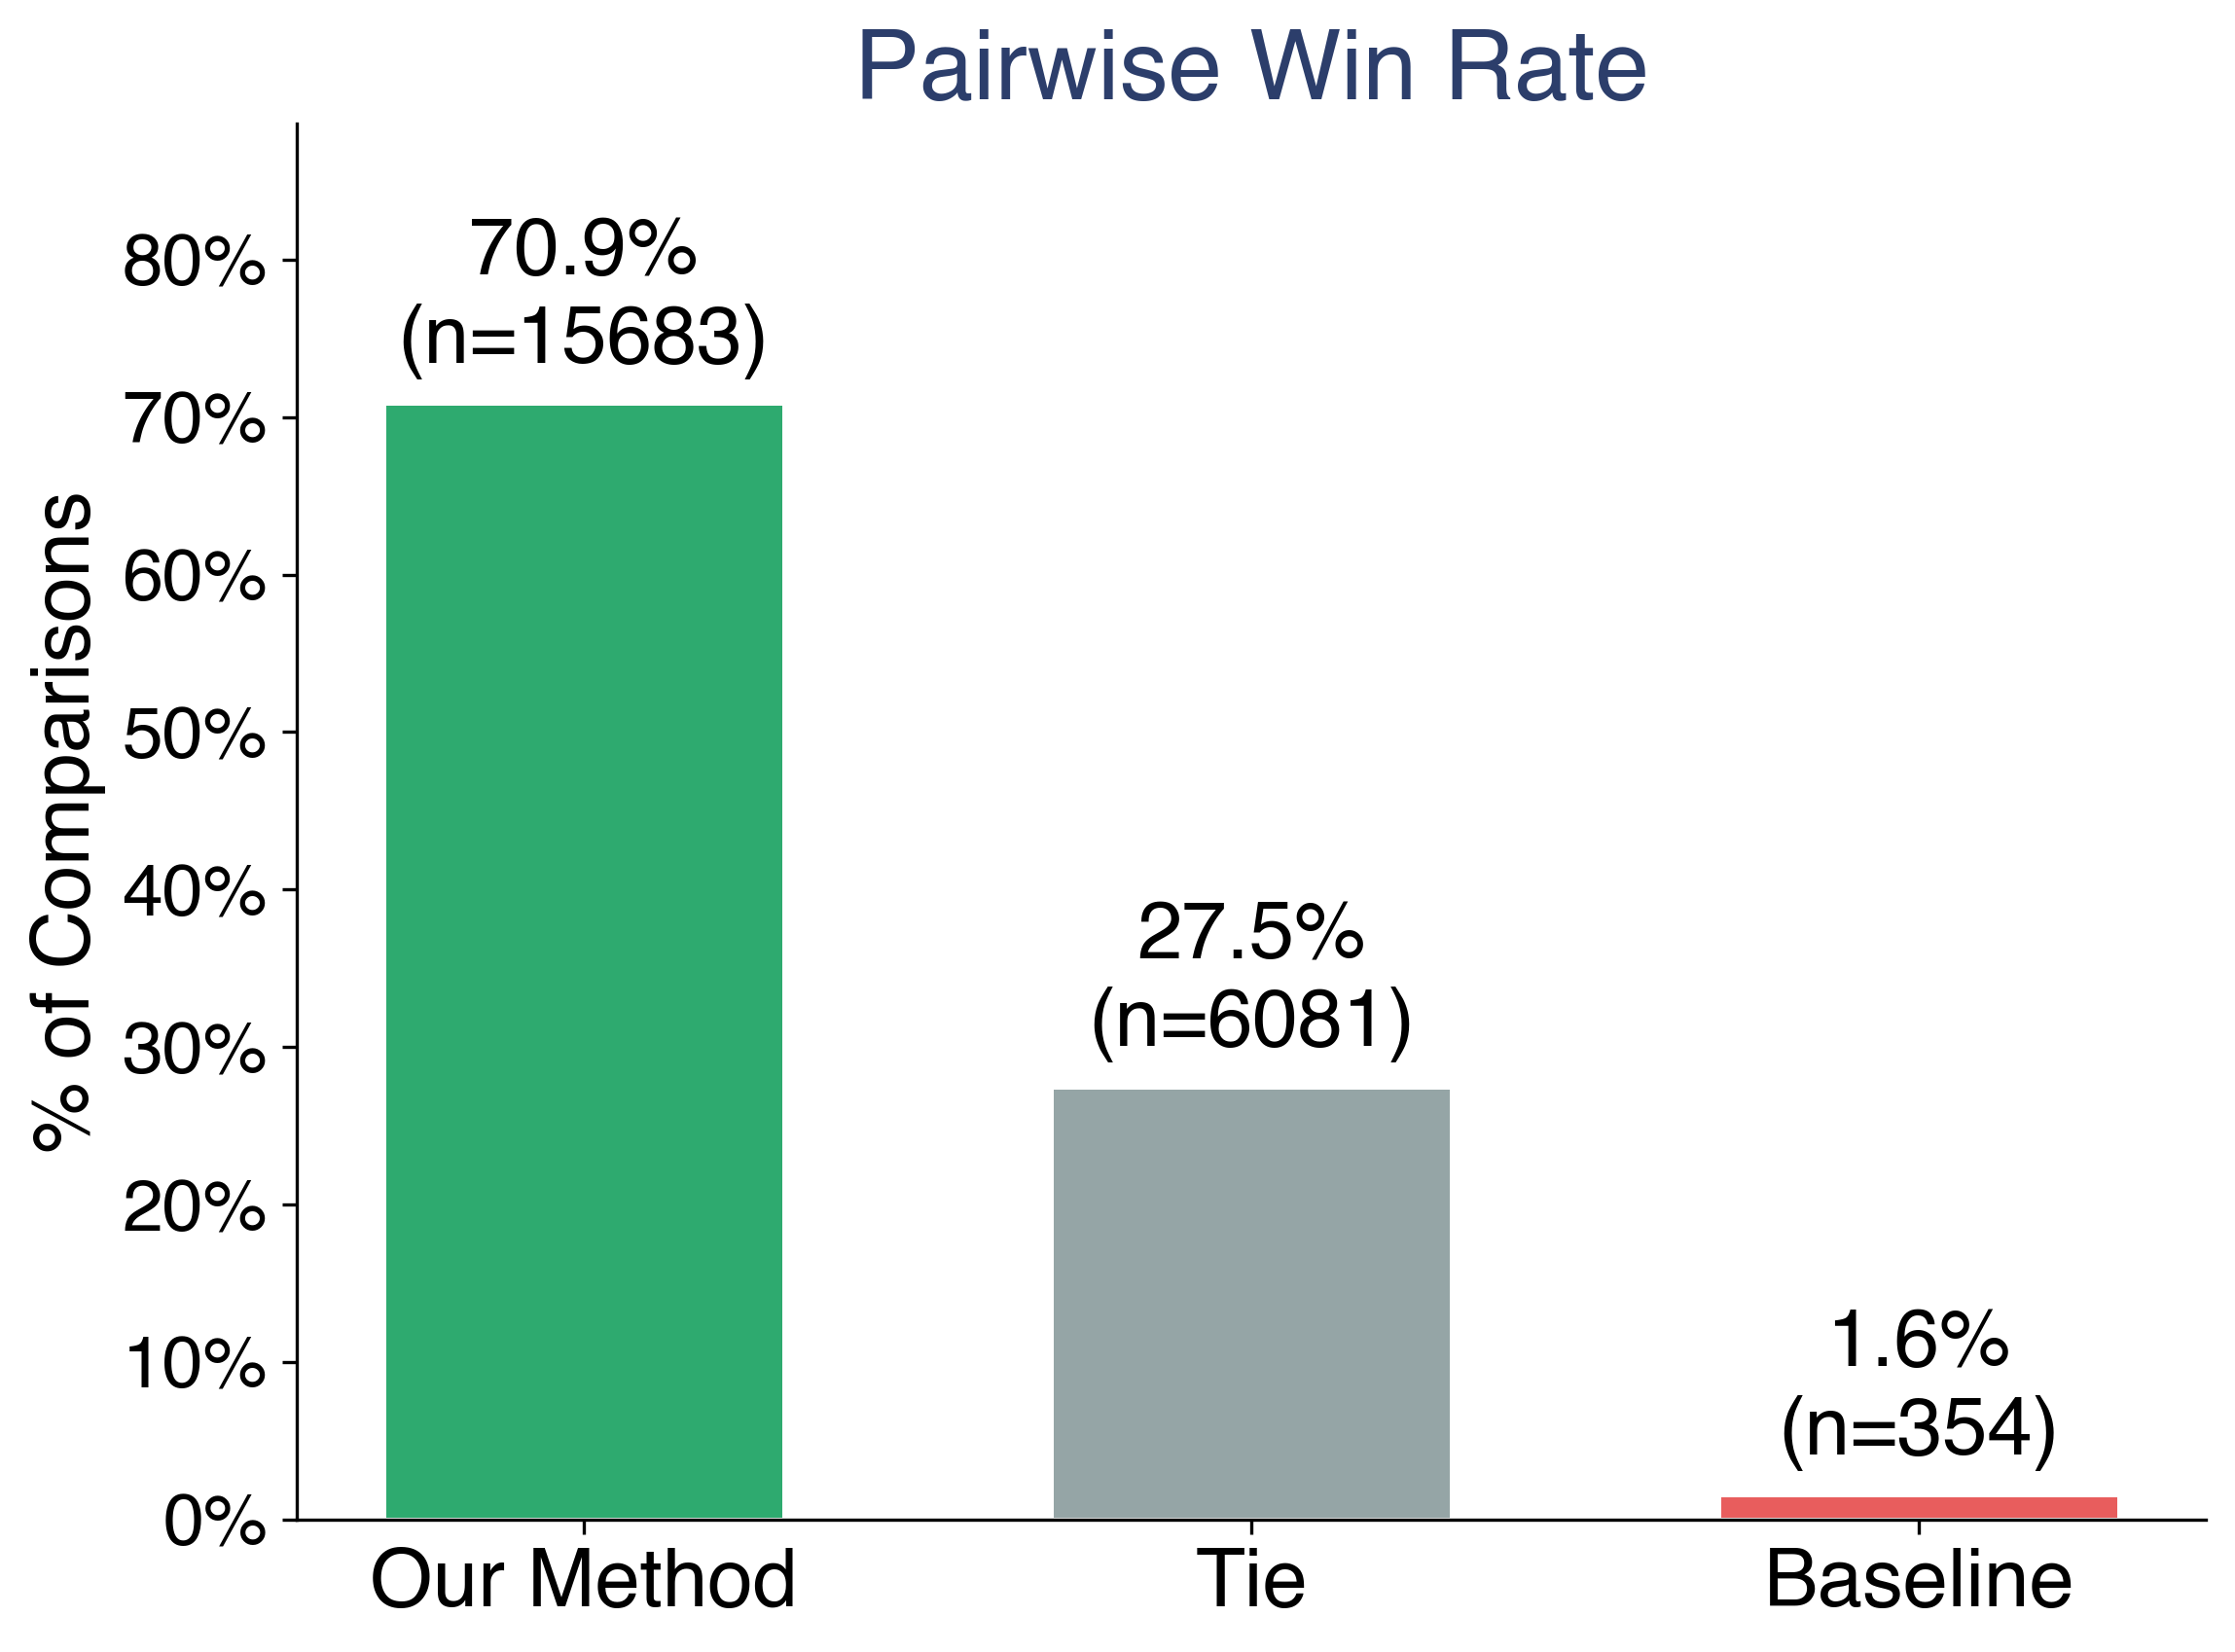
\includegraphics[width=\linewidth]{win_rate.png}
\end{minipage}
\hfill
\begin{minipage}[t]{0.48\linewidth}
  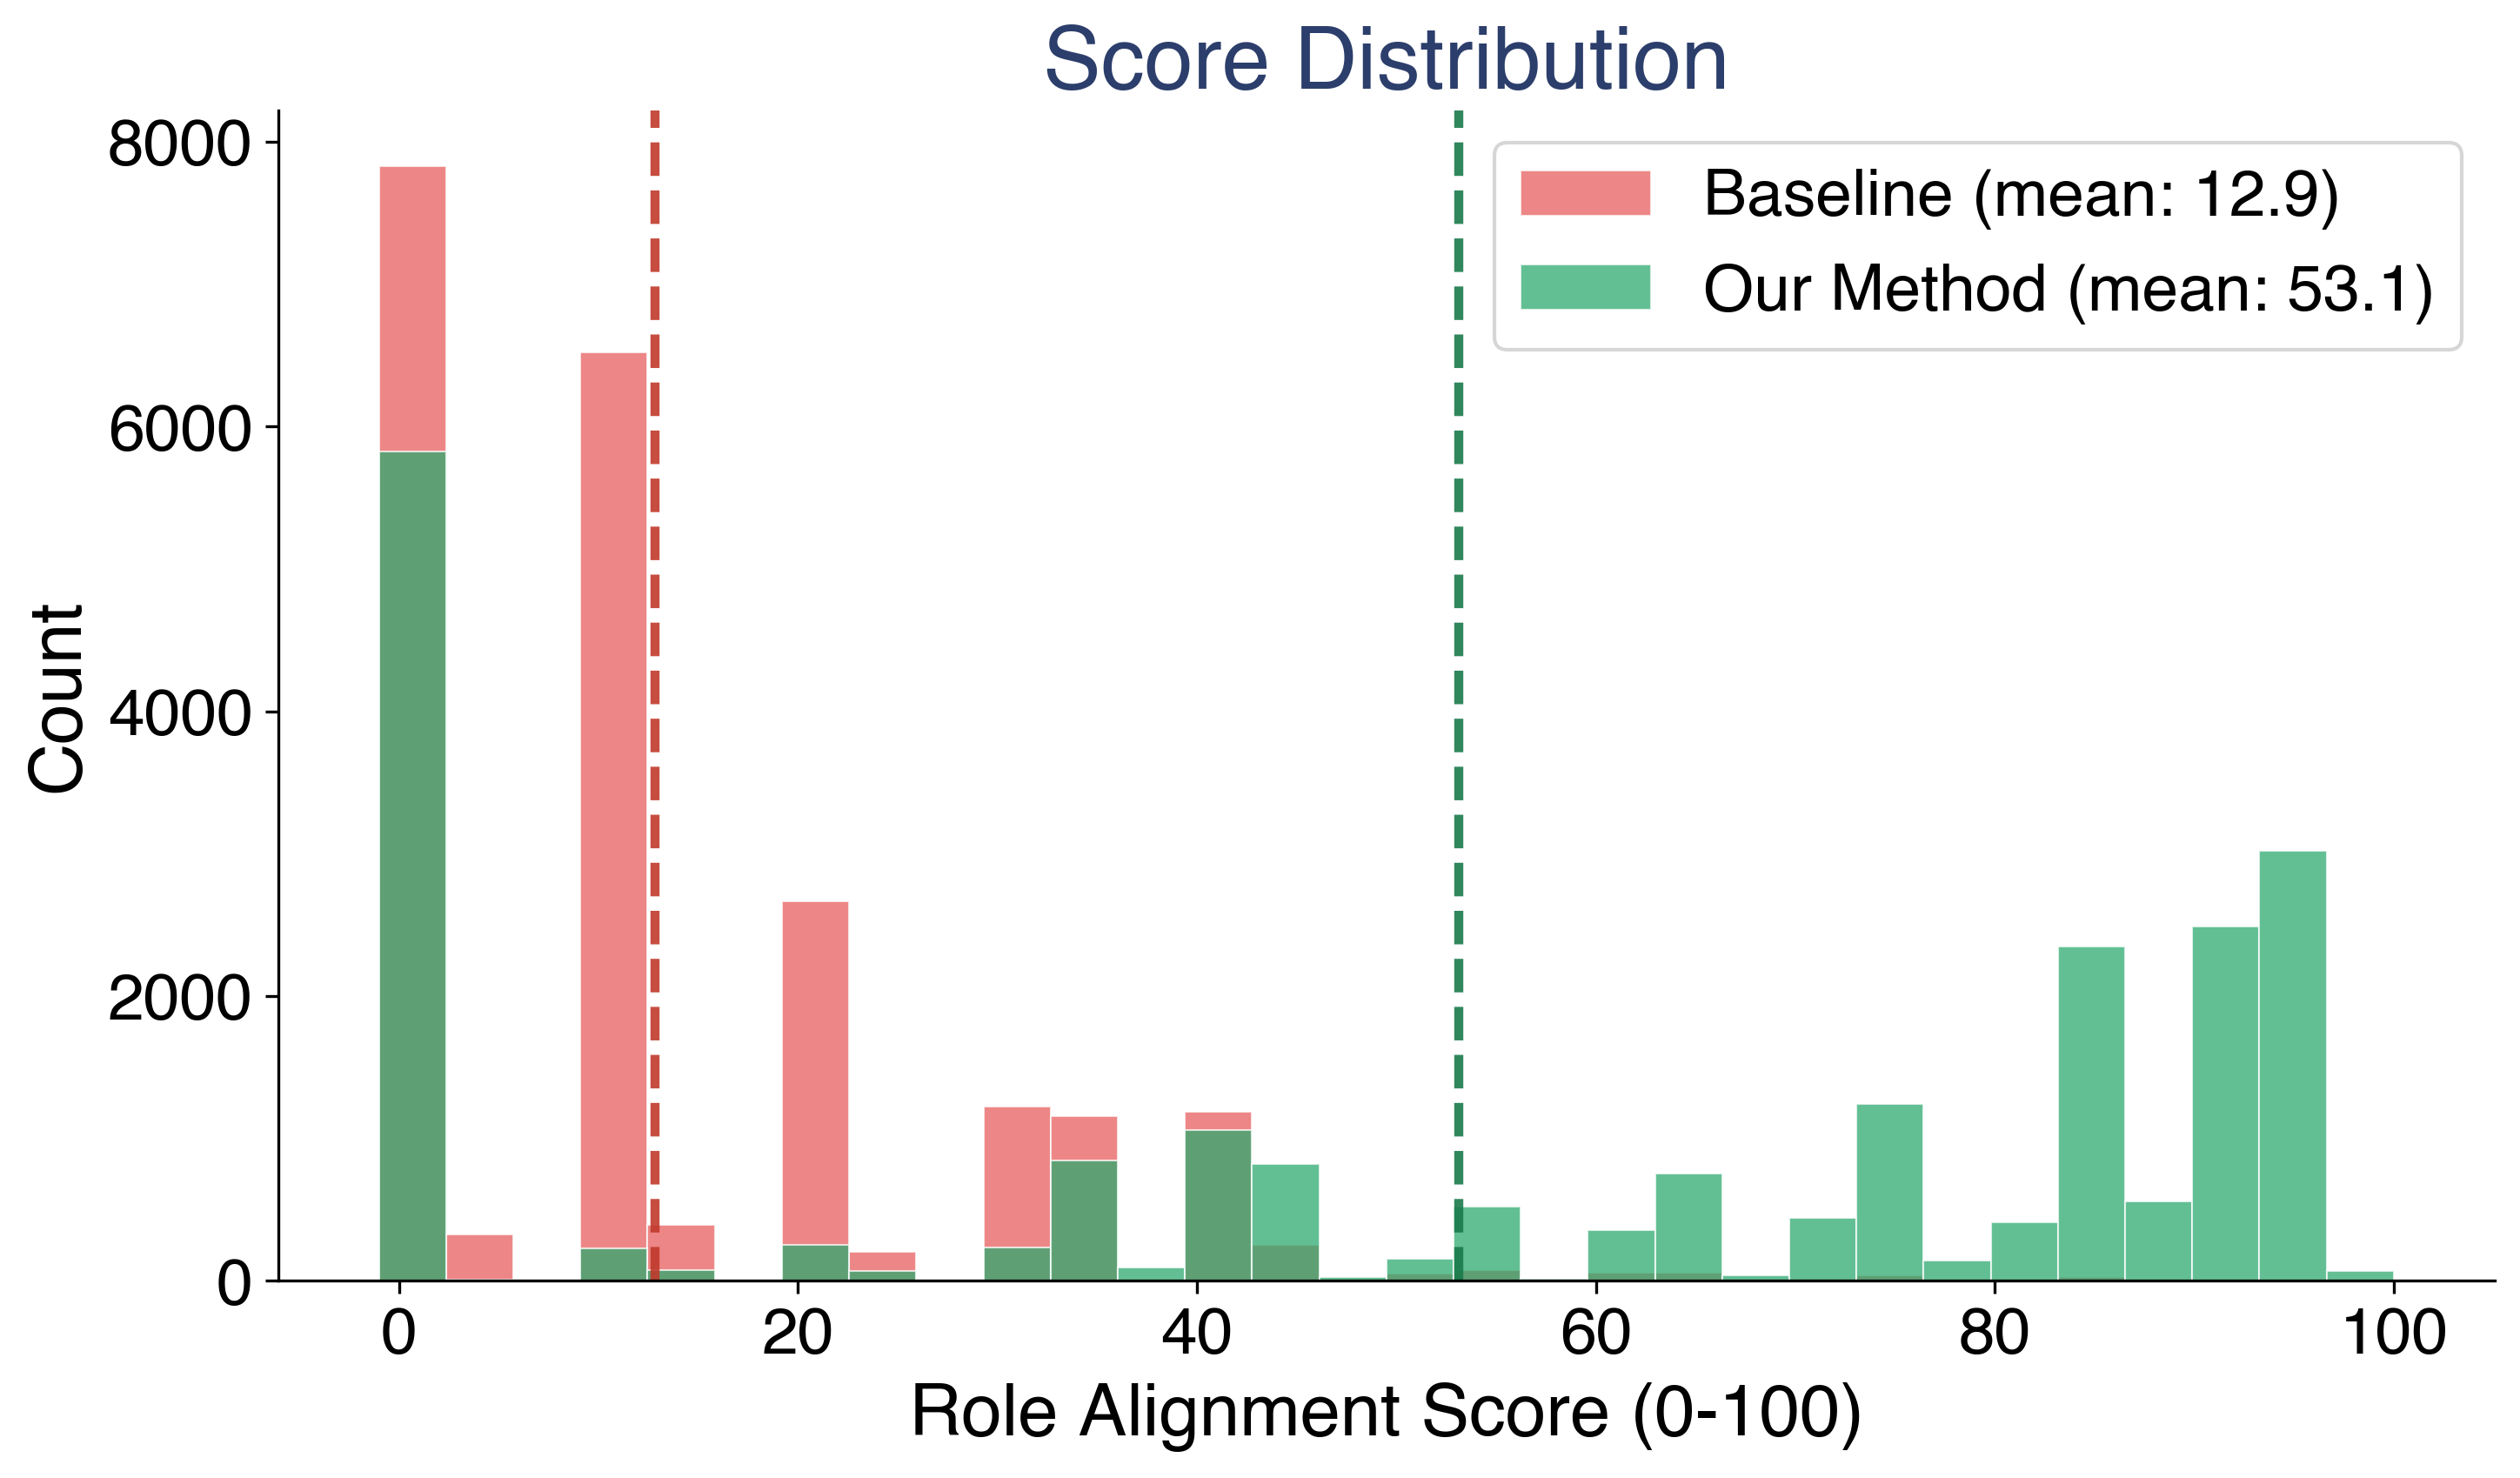
\includegraphics[width=\linewidth]{score_distribution.png}
\end{minipage}

\vspace{2pt}
\begin{hlbox}
\textbf{70.9\%} win rate across 22,118 comparisons
(97 roles). Mean role-alignment score: \textbf{53.1}
(ours) vs.\ \textbf{12.9} (baseline). We lead on all
97 evaluated roles with zero losses.
\end{hlbox}
\end{block}

\end{column}

% ══════════════════════════════════════════════════════════
% COLUMN 2 (wider)
% ══════════════════════════════════════════════════════════
\begin{column}{0.36\textwidth}

\begin{block}{The Fantastical Separation}
t-SNE visualization of our 275 role vectors reveals two
geometrically distinct clusters that were not anticipated
by our extraction methodology.

The upper cluster contains \textbf{human/realistic roles}:
\textit{doctor, lawyer, pirate, mechanic, historian,
economist, comedian, spy, facilitator, judge}.
The lower cluster contains \textbf{fantastical and non-human roles}:
\textit{avatar, eldritch, alien, angel, mystic, symbiote,
shaman, whale, coral reef, revenant}. Notably, \textit{toddler}
and \textit{infant} cluster with this group, suggesting the
model treats pre-linguistic entities as distinct from adult
conversational personas.

To validate this separation, we independently rated each role's
``mystical-ness'' (0--10) using a separate LLM evaluator.
The resulting scores align with the cluster boundaries,
suggesting the separation reflects meaningful semantic structure.

\vspace{4pt}
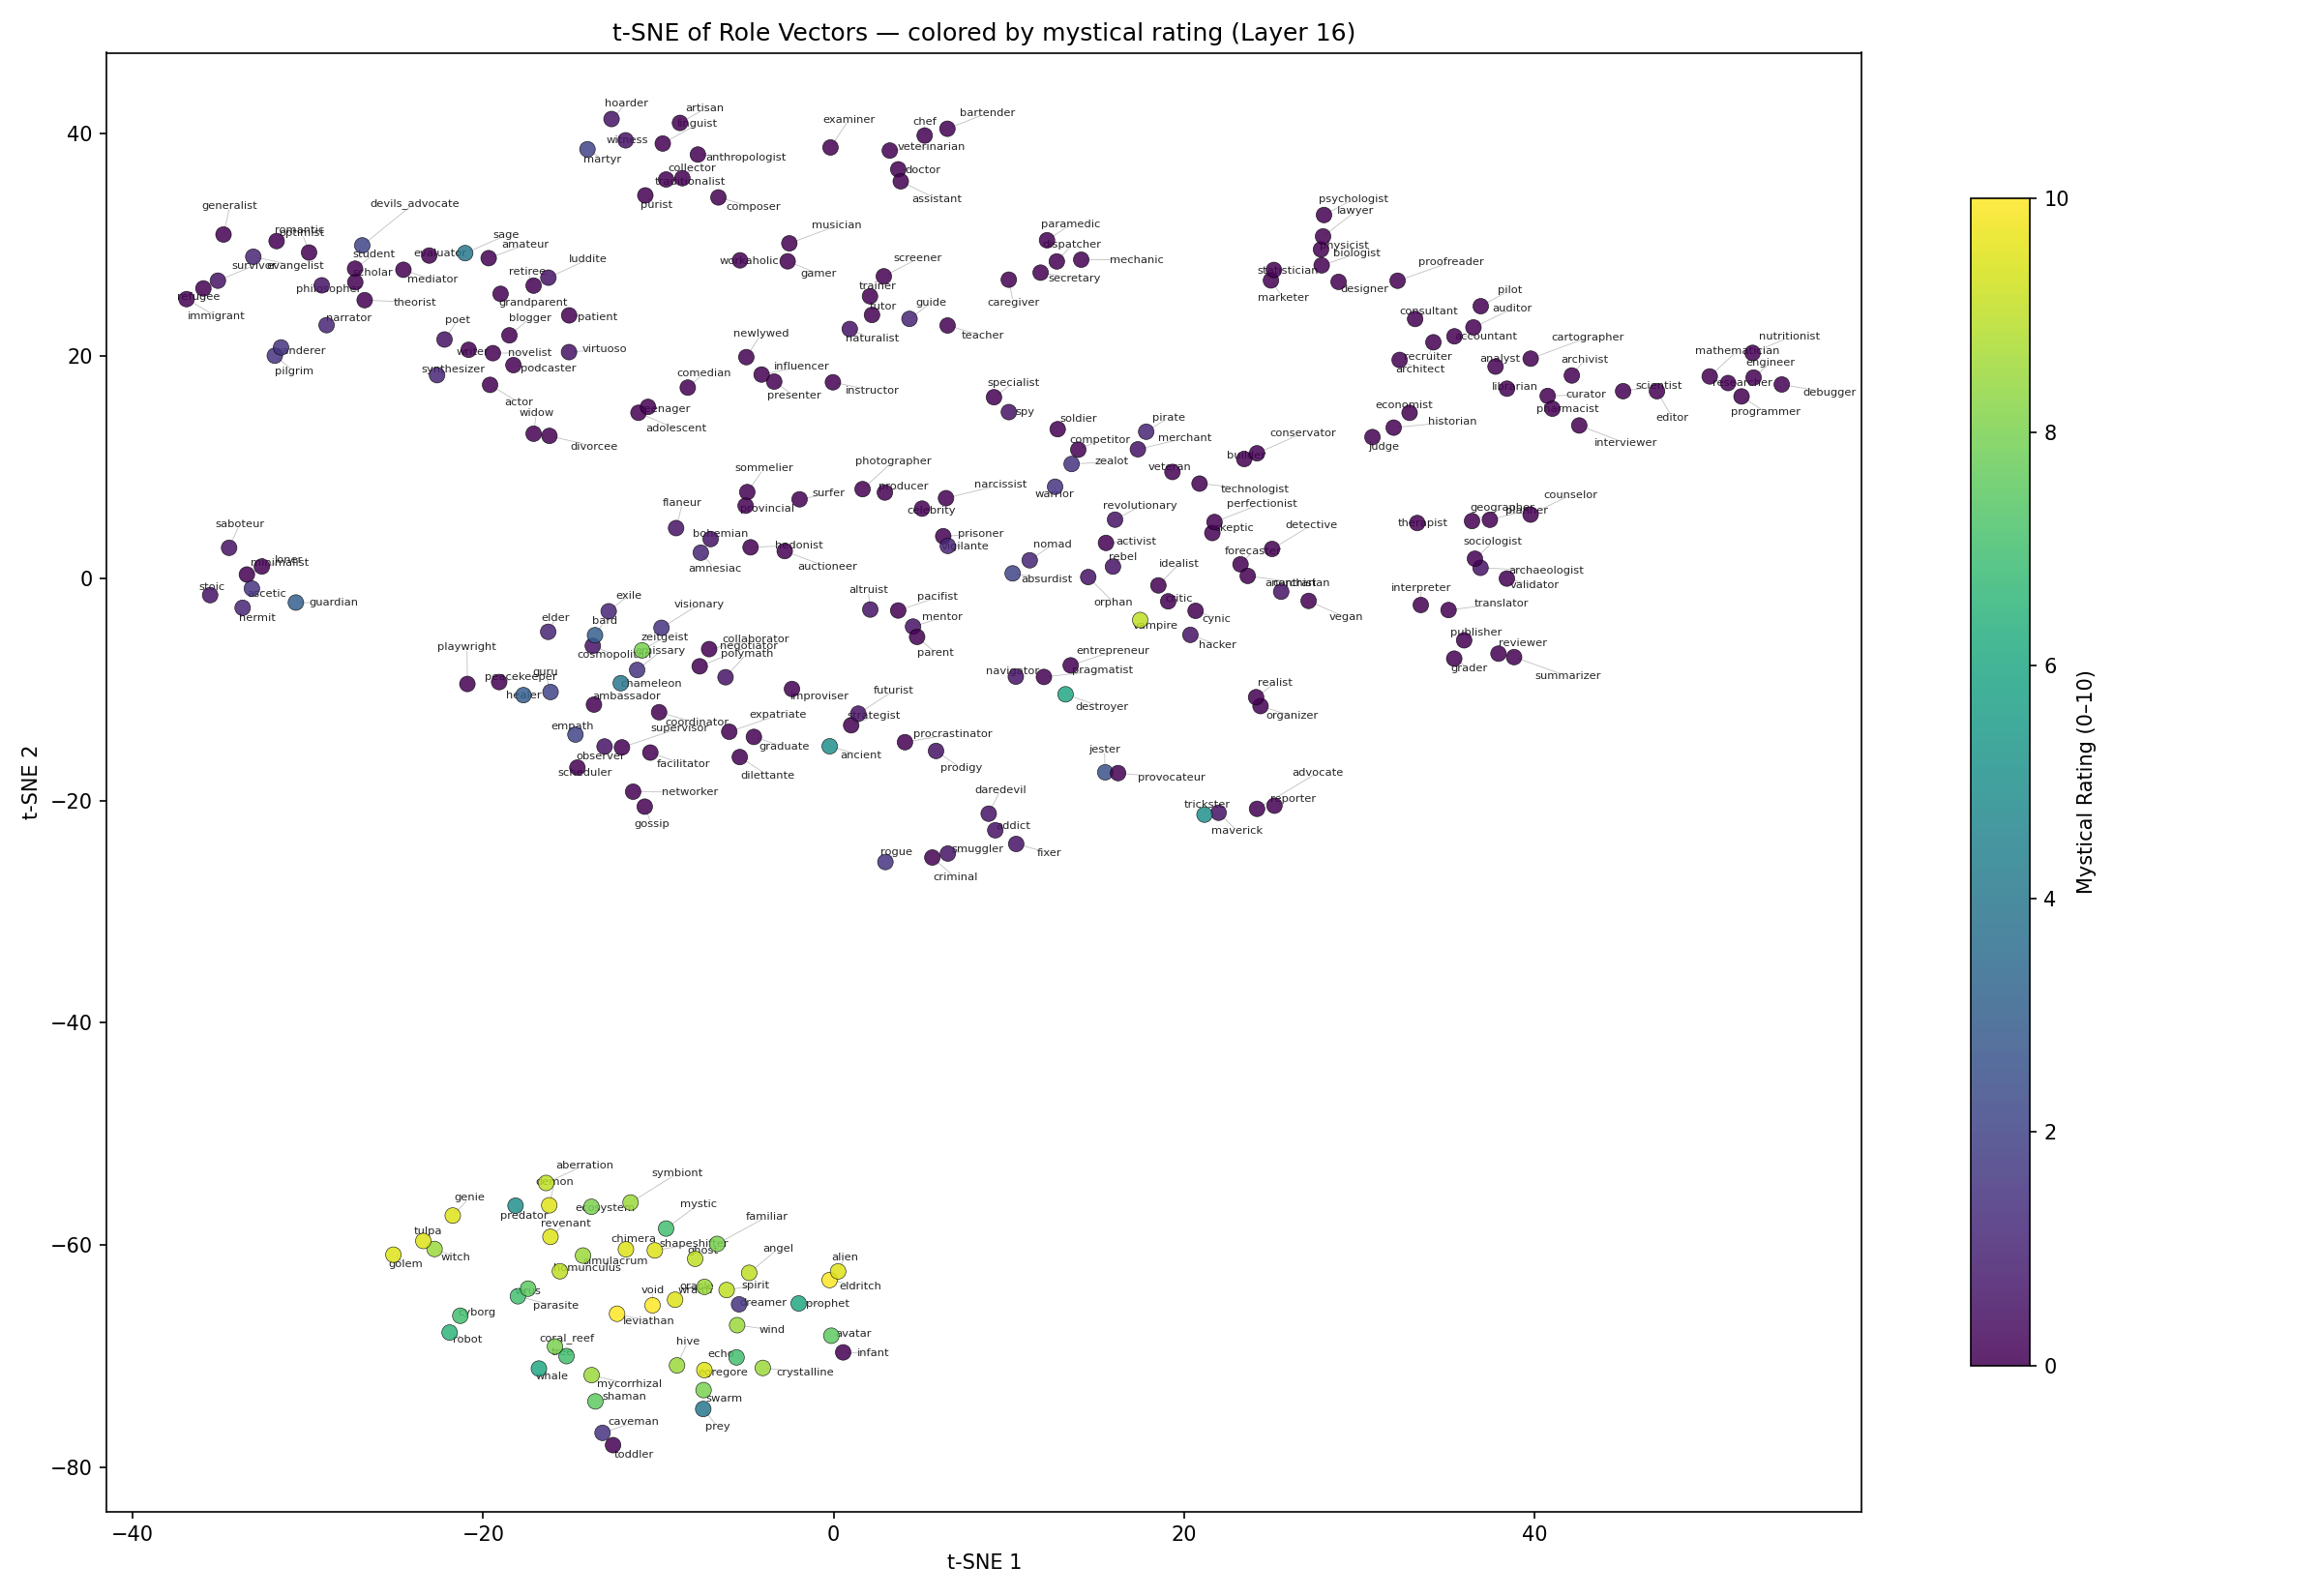
\includegraphics[width=\linewidth]{role_colored_tsne_mystical_layer_16.png}

{\scriptsize\textit{t-SNE of 275 role vectors (layer 16), colored by
independently-rated mystical score (0--10). The lower cluster
contains fantastical and non-human roles. Perplexity = 5.}}
\end{block}

\begin{block}{Baseline: No Fantastical/Realistic Separation}
We replicate the Assistant Axis methodology [1] and apply the
same t-SNE visualization. The baseline vectors---extracted via
mean activation with mean subtraction---do \textbf{not} exhibit
analogous cluster separation. Roles are distributed without
a clear fantastical/realistic divide.

Both methods operate in the same 4,096-dim activation space.
Our contrastive extraction with judge filtering recovers
role-specific structure that mean-activation methods do not.

\vspace{4pt}
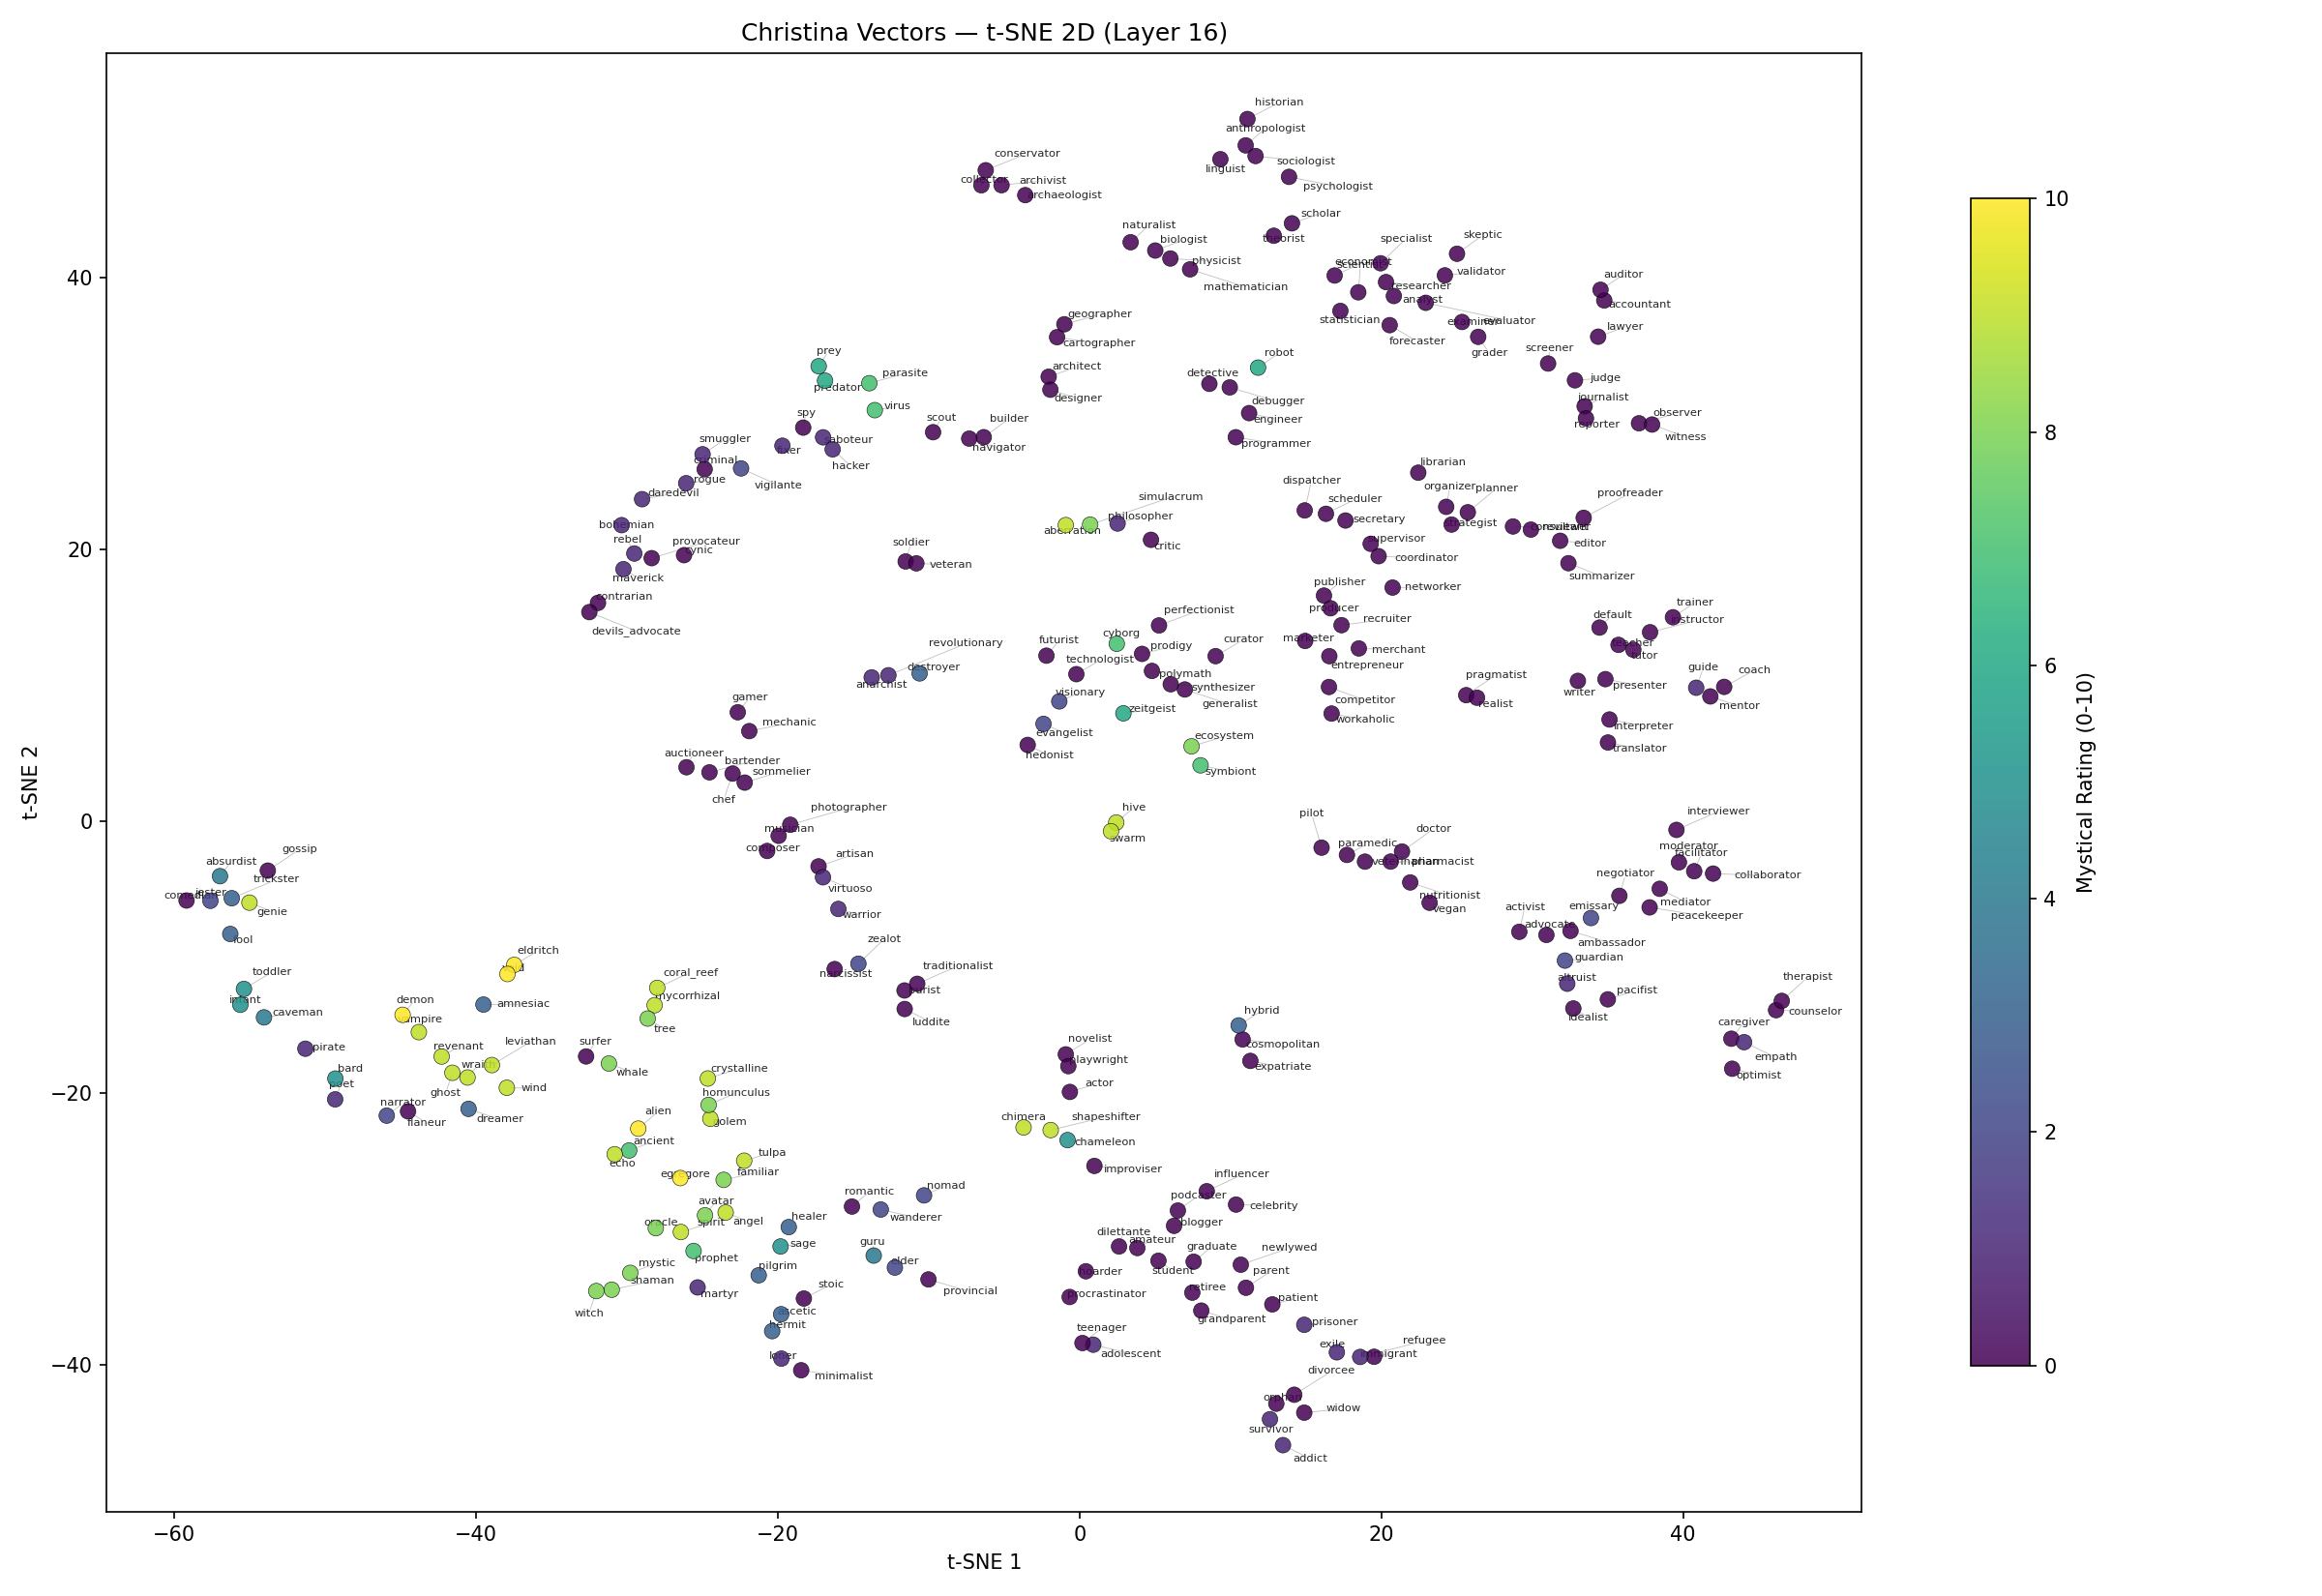
\includegraphics[width=\linewidth]{christina_tsne_mystical.png}

{\scriptsize\textit{Baseline t-SNE (Lu et al.\ [1]), colored by the
same mystical rating scale as our t-SNE above. Mystical
roles (yellow/green) are scattered throughout with no cluster
separation. Same roles, same t-SNE parameters.}}
\end{block}

\end{column}

% ══════════════════════════════════════════════════════════
% COLUMN 3
% ══════════════════════════════════════════════════════════
\begin{column}{0.28\textwidth}

\begin{block}{Geometric Analysis}
PCA on the role vector matrix reveals low-dimensional structure:
${\sim}20$ principal components capture 90\% of variance across
275 roles in 4,096-dim space.

PC1 (associated with the assistant axis [1]) explains 24.0\%
of variance in our vectors vs.\ 25.8\% in the baseline.
Our method distributes variance more evenly across components,
consistent with greater inter-role separability.

\vspace{3pt}
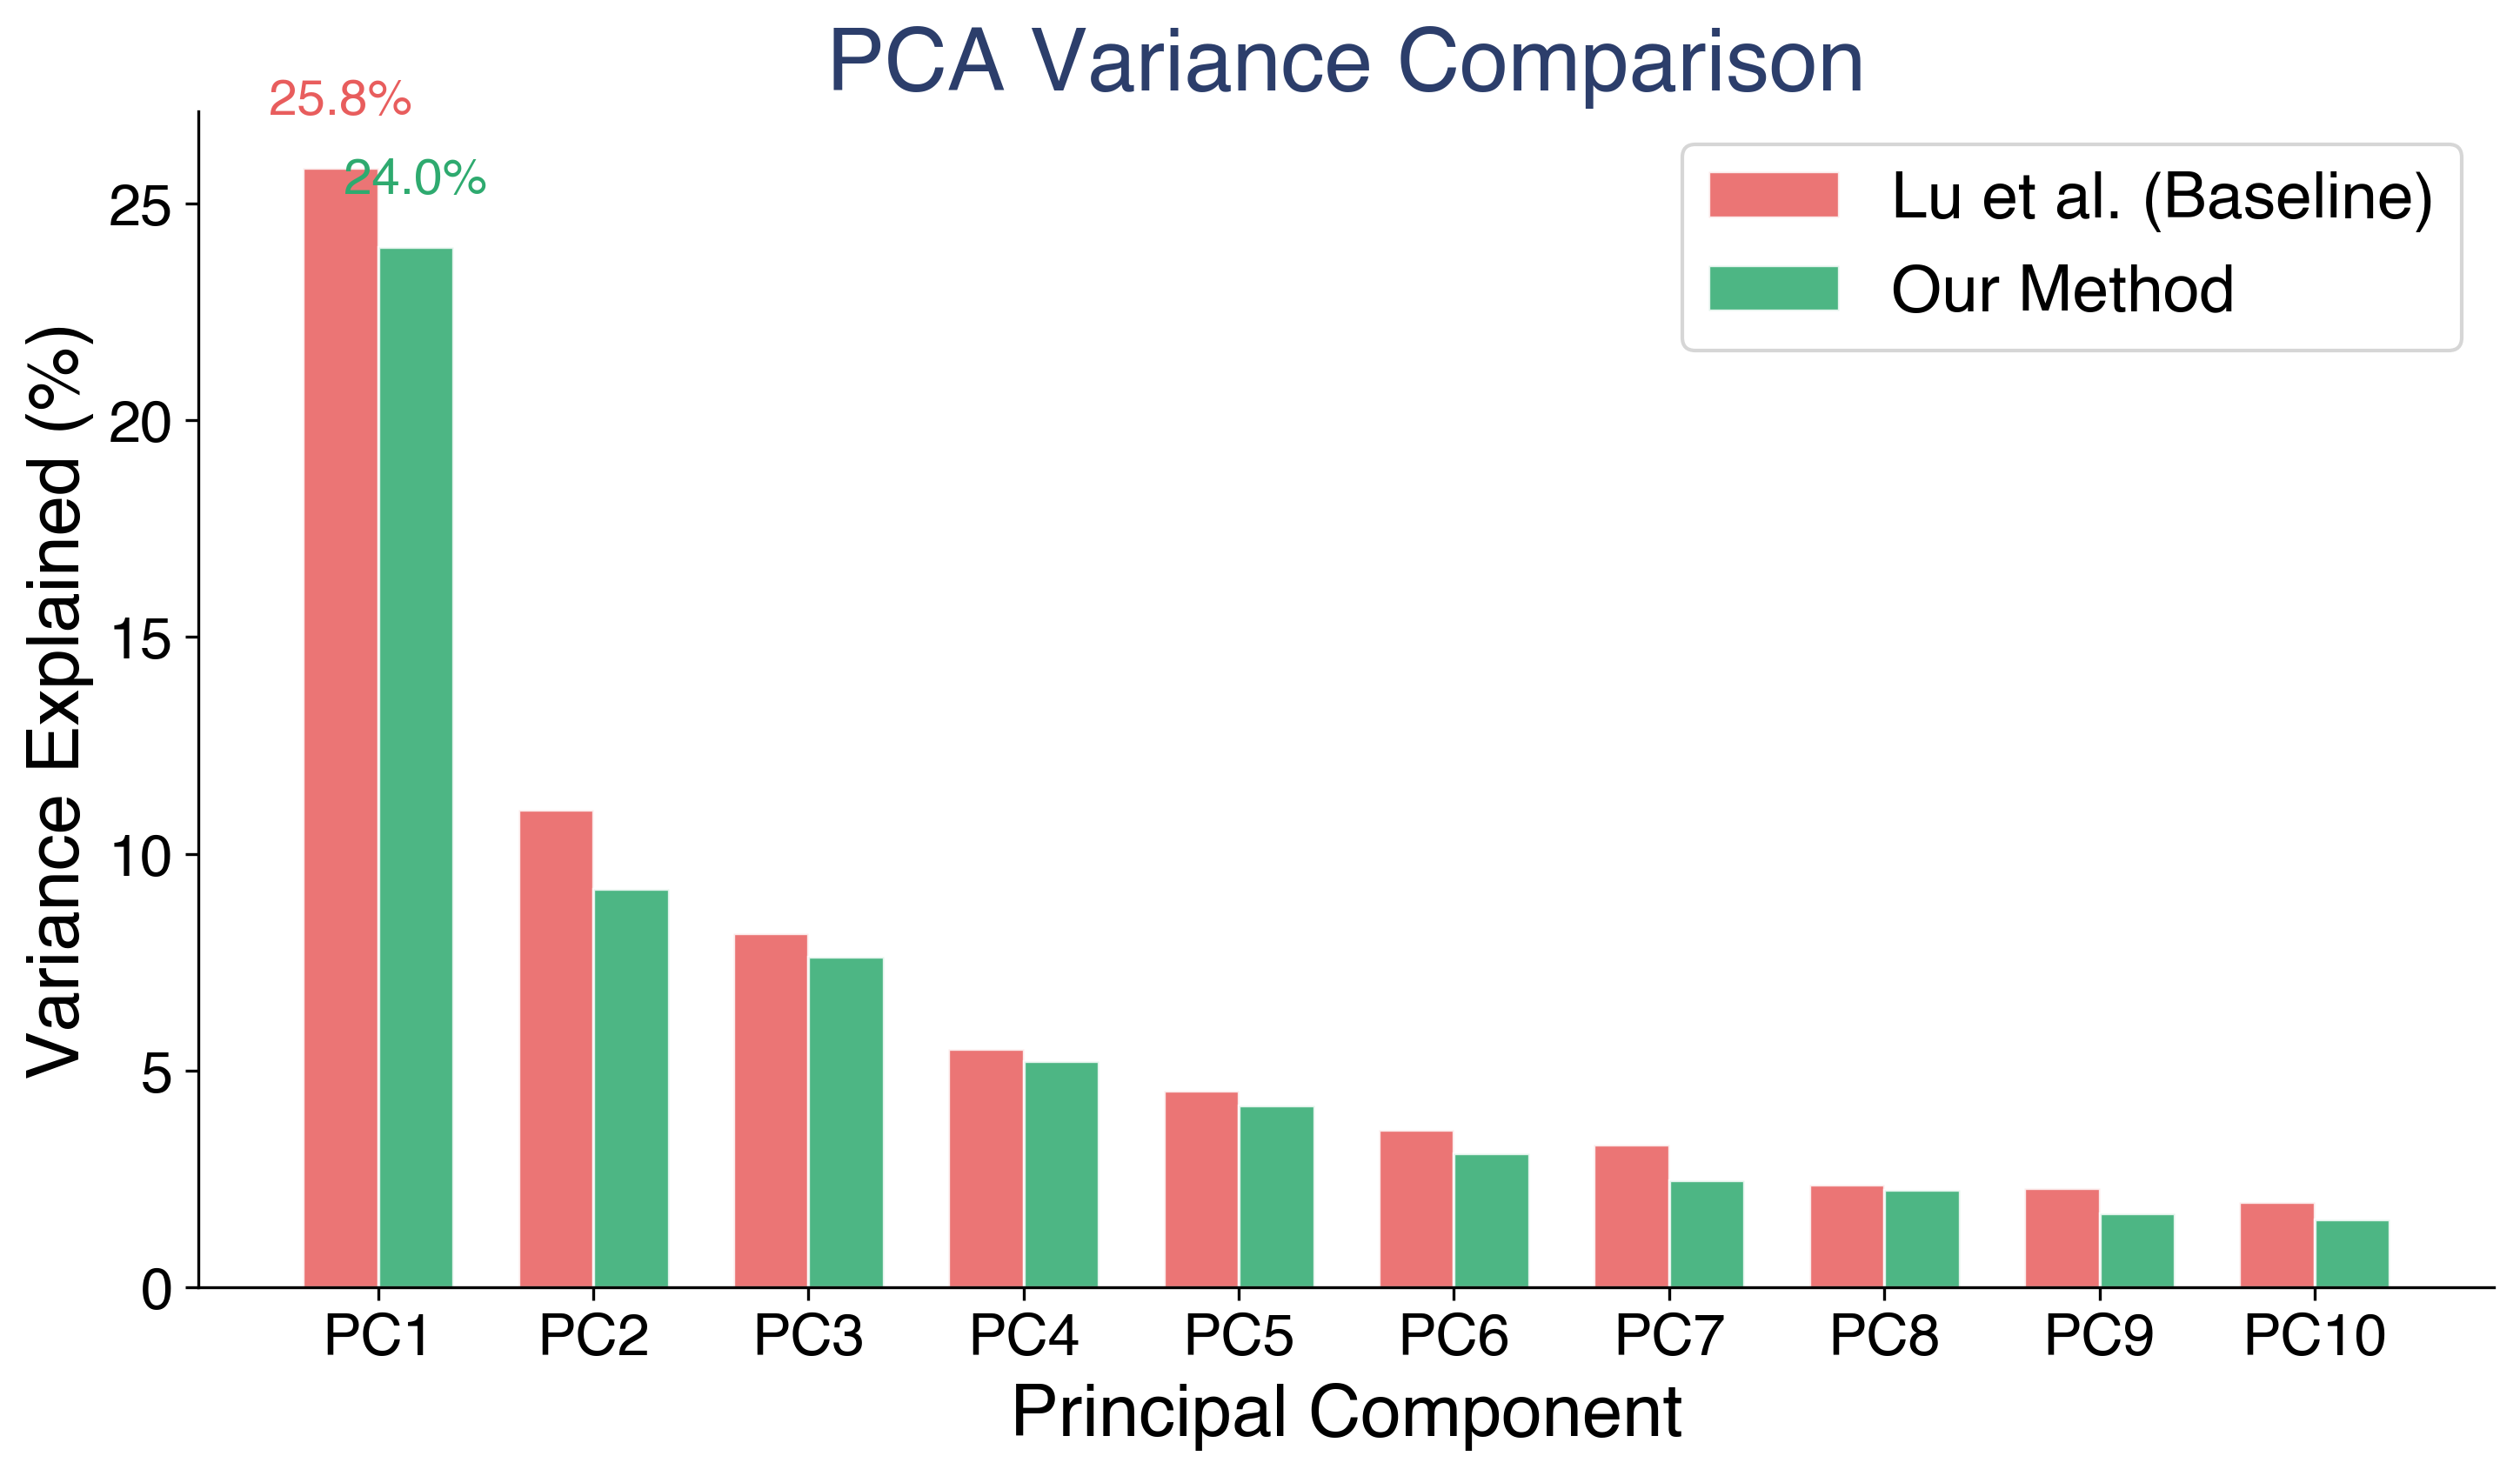
\includegraphics[width=\linewidth]{pca_variance_comparison.png}

{\scriptsize\textit{Variance explained per principal component.
Lower PC1 concentration indicates greater separability between
roles. ${\sim}20$ PCs needed for 90\% cumulative variance
(first 10 shown).}}
\end{block}

\begin{block}{PCA Supports Cluster Structure}
To test whether the t-SNE finding persists in the raw geometry,
we construct a custom 3D basis: the assistant axis as dimension
1, with two residual PCA components as dimensions 2 and 3.
High-mystical roles occupy a distinct region along the residual
axes, indicating the cluster is present beyond t-SNE.

\vspace{3pt}

\includegraphics[width=\linewidth]{role_colored_pca_mystical_layer_16.png}

{\scriptsize\textit{3D PCA colored by mystical rating. The assistant
axis (dashed) defines dimension 1. Fantastical roles
(yellow/green) cluster in the upper region of the residual
space, separated from realistic roles.}}

\end{block}

\begin{block}{Vector Arithmetic}
Role vectors support algebraic composition analogous to word
embedding arithmetic [6], suggesting the space encodes
relational structure between personas:

\vspace{4pt}
{\centering\small
\textbf{warrior} $-$ \textbf{stoic} $+$ \textbf{pacifist}\\
$\approx$ \textit{activist, evangelist, coordinator}\\[3pt]
\textbf{scientist} $-$ \textbf{critic} $+$ \textbf{criminal}\\
$\approx$ \textit{smuggler, hacker, detective}\\
}

\vspace{3pt}
{\scriptsize Nearest neighbors by cosine similarity. These
results suggest compositional structure but require
further systematic validation.}
\end{block}

\end{column}

\end{columns}

\vspace{0mm}

% ── CONCLUSIONS ─────────────────────────────────────────────
\begin{block}{Conclusions \& Future Work}
\begin{columns}[T]
\begin{column}{0.42\textwidth}
\begin{itemize}[leftmargin=1em, itemsep=2pt, topsep=0pt, parsep=0pt, label=$\bullet$]
  \item \textbf{Contrastive extraction with judge filtering} wins
    70.9\% of comparisons against the Assistant Axis baseline [1]
    across 97 roles (22,118 comparisons, 500k+ Q/A pairs),
    with mean score 53.1 vs.\ 12.9. Zero role-level losses.
  \item \textbf{Fantastical/non-human roles} occupy a
    geometrically distinct subspace, visible in both t-SNE and
    PCA, with boundaries aligned to an independent mystical
    rating. Pre-linguistic roles cluster with this group.
  \item Role space exhibits \textbf{low-dimensional structure}
    (${\sim}20$ PCs for 90\% variance) and suggestive algebraic
    compositionality. Our fantastical/realistic separation
    mirrors the PC1 axis found across three other models [1],
    providing converging evidence for the Persona Selection
    Model [9].
  \item \textbf{Future work:} Full 275-role evaluation,
    k-means verification, cross-model generalization [5].
\end{itemize}
\end{column}
\begin{column}{0.50\textwidth}
{\small\textbf{References}}\\[1pt]
{\scriptsize
{[1]} Lu et al.\ (2026). \textit{The Assistant Axis.}
{[2]} Chen et al.\ (2024). \textit{From Persona to Personalization.}
{[3]} Panickssery et al.\ (2023). \textit{Steering via Contrastive Activation Addition.}
{[4]} Zou et al.\ (2023). \textit{Representation Engineering.}
{[5]} Wang et al.\ (2025). \textit{Persona Features Control Emergent Misalignment.}
{[6]} Wang et al.\ (2023). \textit{RoleLLM.}
{[7]} Tan et al.\ (2024). \textit{Generalization of Steering Vectors.}
{[8]} Li et al.\ (2024). \textit{Instruction (In)Stability in LM Dialogs.}
{[9]} Anthropic (2026). \textit{The Persona Selection Model.}\\[2pt]
}
{\small\textbf{Acknowledgments}}\\[1pt]
{\scriptsize
This work was supported in part by a gift from Charles Frye of Modal.
We thank Sumuk Shashidhar and the following for peer review and
feedback: A.~Singh, C.~Lu, C.~Ackerman, D.~Ivanova,
D.~D.~Africa, G.~Kroiz, J.~Chooi, J.~Heninger, J.~Michala,
N.~Warncke, R.~Dearnaley, R.~Kidd, T.~Hua.
}
\end{column}
\end{columns}
\end{block}

\end{frame}
\end{document}
